\begin{tomtat}
	\begin{minipage}[t]{0.3\textwidth}
		\vspace{0pt}
		\begin{tomtat}
			\begin{center}
				\textbf{ĐỀ 14}
			\end{center}
			
		\end{tomtat}
	\end{minipage}
	\hfill
	\begin{minipage}[t]{0.5\textwidth}
		\vspace{0pt}
		\begin{tomtat}
			\begin{center}
				\includegraphics[scale=0.08]{images/14}
			\end{center}
		\end{tomtat}
	\end{minipage}
\end{tomtat}
\textbf{I. PHẦN TRẮC NGHIỆM}
\begin{ex} % Câu 1
	Giá trị của biểu thức $A=\sqrt{50}-\sqrt{2}$ là:
	\choice{$2\sqrt{2}$}{$3\sqrt{2}$}{$4\sqrt{2}$}{$-4\sqrt{2}$}
	\loigiai{
		Ta có:
		\begin{align*}
			A &= \sqrt{50}-\sqrt{2} \\
			&= \sqrt{25 \cdot 2} - \sqrt{2} \\
			&= 5\sqrt{2} - \sqrt{2} \\
			&= (5-1)\sqrt{2} \\
			&= 4\sqrt{2}
		\end{align*}
		\\ \textbf{ĐÁP ÁN C}
	}
\end{ex}

\begin{ex} % Câu 2
	Giải bất phương trình $-x-3>0$ ta được nghiệm là:
	\choice{$x>3$}{$x>-3$}{$x<-3$}{$x<3$}
	\loigiai{
		Ta giải bất phương trình:
		\begin{align*}
			-x-3 &> 0 \\
			-x &> 3
		\end{align*}
		Nhân cả hai vế của bất phương trình với -1 và đổi chiều bất đẳng thức:
		\begin{align*}
			x &< -3
		\end{align*}
		Vậy nghiệm của bất phương trình là $x<-3$.
		\\ \textbf{ĐÁP ÁN C}
	}
\end{ex}

\begin{ex} % Câu 3
	Giá trị của hàm số $y = f(x) = \frac{4}{5}x^2$ tại $x_0 = -5$ là:
	\choice{$-20$}{$20$}{$-5$}{$5$}
	\loigiai{
		Thay $x_0 = -5$ vào hàm số $y = \frac{4}{5}x^2$:
		\begin{align*}
			y &= \frac{4}{5}(-5)^2 \\
			&= \frac{4}{5}(25) \\
			&= 4 \cdot \frac{25}{5} \\
			&= 4 \cdot 5 \\
			&= 20
		\end{align*}
		Vậy giá trị của hàm số tại $x_0 = -5$ là 20.
		\\ \textbf{ĐÁP ÁN B}
	}
\end{ex}

\begin{ex} % Câu 4
	Một xạ thủ bắn 40 phát kết quả như sau:
	\begin{center}
		\begin{tabular}{|l|c|c|c|c|}
			\hline
			Điểm & 7 & 8 & 9 & 10 \\
			\hline
			Tần số & 8 & ? & 10 & 8 \\
			\hline
		\end{tabular}
	\end{center}
	Tần số của điểm 8 là:
	\choice{12}{13}{14}{15}
	\loigiai{
		Tổng số phát bắn là 40.
		Tổng tần số của các điểm đã biết là:
		Tần số điểm 7: 8
		Tần số điểm 9: 10
		Tần số điểm 10: 8
		Tổng các tần số đã biết = $8 + 10 + 8 = 26$.
		Tần số của điểm 8 là:
		$40 - (\text{Tổng các tần số đã biết})$
		$= 40 - 26 = 14$.
		\\ \textbf{ĐÁP ÁN C}
	}
\end{ex}

\begin{ex} % Câu 5
	Bạn Nam gieo một con xúc xắc 10 lần liên tiếp thì thấy mặt 4 chấm xuất hiện 3 lần. Xác suất thực nghiệm xuất hiện mặt 4 chấm là:
	\choice{$\frac{3}{10}$}{$\frac{4}{10}$}{$\frac{7}{10}$}{$\frac{3}{14}$}
	\loigiai{
		Xác suất thực nghiệm của một biến cố được tính bằng tỉ số giữa số lần biến cố đó xảy ra và tổng số lần thực hiện phép thử.
		Số lần gieo xúc xắc (tổng số lần thực hiện phép thử) là $N = 10$ lần.
		Số lần mặt 4 chấm xuất hiện (số lần biến cố xảy ra) là $k = 3$ lần.
		Xác suất thực nghiệm xuất hiện mặt 4 chấm là:
		$$ P(\text{mặt 4 chấm}) = \frac{k}{N} = \frac{3}{10} $$
		\\ \textbf{ĐÁP ÁN A}
	}
\end{ex}

\begin{ex} % Câu 6
	Cho tam giác ABC vuông tại A, có AB=12cm, BC=15cm. Tính cosB.
	\choice{$\frac{4}{3}$}{$\frac{3}{4}$}{$\frac{4}{5}$}{$\frac{3}{5}$}
	\loigiai{
		Trong tam giác ABC vuông tại A:
		Theo định nghĩa tỉ số lượng giác cosin trong tam giác vuông, ta có:
		$$ \cos B = \frac{\text{cạnh kề}}{\text{cạnh huyền}} = \frac{AB}{BC} $$
		Với $AB=12 \text{ cm}$ và $BC=15 \text{ cm}$, ta có:
		$$ \cos B = \frac{12}{15} $$
		Rút gọn phân số:
		$$ \cos B = \frac{12 \div 3}{15 \div 3} = \frac{4}{5} $$
		\\ \textbf{ĐÁP ÁN C}
	}
\end{ex}

\begin{ex} % Câu 7
	Phương trình: $-3x+5=11$ có nghiệm là:
	\choice{$x=-2$}{$x=2$}{$x=\frac{16}{3}$}{$x=\frac{-16}{3}$}
	\loigiai{
		Ta giải phương trình:
		\begin{align*}
			-3x+5 &= 11 \\
			-3x &= 11-5 \\
			-3x &= 6 \\
			x &= \frac{6}{-3} \\
			x &= -2
		\end{align*}
		Vậy nghiệm của phương trình là $x=-2$.
		\\ \textbf{ĐÁP ÁN A}
	}
\end{ex}
\begin{ex} % Câu 8 (từ ảnh mới)
	Cho hình nón có bán kính đáy bằng 4cm, độ dài đường sinh là 10 cm. Tính diện tích xung quanh của hình nón đó là:
	\choice{$20\pi \text{ cm}^2$}{$160\pi \text{ cm}^2$}{$30\pi \text{ cm}^2$}{$40\pi \text{ cm}^2$}
	\loigiai{
		Diện tích xung quanh của hình nón được tính bằng công thức: $S_{xq} = \pi Rl$.
		Trong đó:
		$R$ là bán kính đáy của hình nón.
		$l$ là độ dài đường sinh của hình nón.
		Theo đề bài, $R = 4 \text{ cm}$ và $l = 10 \text{ cm}$.
		\begin{align*}
			S_{xq} &= \pi \cdot R \cdot l \\
			&= \pi \cdot 4 \cdot 10 \\
			&= 40\pi \text{ (cm}^2\text{)}
		\end{align*}
		\\ \textbf{ĐÁP ÁN D}
	}
\end{ex}
\newpage
\textbf{II. PHẦN TỰ LUẬN}
\begin{ex} % Câu 9
	Giải hệ phương trình: $\begin{cases} 2x+y=5 \\ x-3y=-1 \end{cases}$
	\loigiai{
		Ta có hệ phương trình:
		$$ \begin{cases} 2x+y=5 & (1) \\ x-3y=-1 & (2) \end{cases} $$
		Từ phương trình (1), suy ra $y = 5-2x$.
		Thay $y = 5-2x$ vào phương trình (2):
		\begin{align*}
			x - 3(5-2x) &= -1 \\
			x - 15 + 6x &= -1 \\
			7x &= -1 + 15 \\
			7x &= 14 \\
			x &= 2
		\end{align*}
		Thay $x=2$ vào $y = 5-2x$:
		\begin{align*}
			y &= 5 - 2(2) \\
			y &= 5 - 4 \\
			y &= 1
		\end{align*}
		Vậy nghiệm của hệ phương trình là $(x; y) = (2; 1)$.
	}
\end{ex}

\begin{ex} % Câu 10 (Rút gọn)
	Rút gọn biểu thức $P=\frac{2}{\sqrt{x}+1}+\frac{2}{\sqrt{x}-1}+\frac{\sqrt{x}-5}{x-1}$ với $x \ge 0, x \ne 1$.
	\loigiai{
		Với $x \ge 0, x \ne 1$, ta có $x-1 = (\sqrt{x}-1)(\sqrt{x}+1)$.
		\begin{align*}
			P &= \frac{2(\sqrt{x}-1)}{(\sqrt{x}+1)(\sqrt{x}-1)} + \frac{2(\sqrt{x}+1)}{(\sqrt{x}-1)(\sqrt{x}+1)} + \frac{\sqrt{x}-5}{(\sqrt{x}-1)(\sqrt{x}+1)} \\
			&= \frac{2\sqrt{x}-2 + 2\sqrt{x}+2 + \sqrt{x}-5}{(\sqrt{x}-1)(\sqrt{x}+1)} \\
			&= \frac{(2\sqrt{x}+2\sqrt{x}+\sqrt{x}) + (-2+2-5)}{x-1} \\
			&= \frac{5\sqrt{x}-5}{x-1} \\
			&= \frac{5(\sqrt{x}-1)}{(\sqrt{x}-1)(\sqrt{x}+1)}
		\end{align*}
		Vì $x \ne 1$ nên $\sqrt{x}-1 \ne 0$. Ta có thể rút gọn $\sqrt{x}-1$.
		\begin{align*}
			P &= \frac{5}{\sqrt{x}+1}
		\end{align*}
		Vậy $P = \frac{5}{\sqrt{x}+1}$.
	}
\end{ex}

\begin{ex} % Câu 10 (Phương trình bậc hai)
	Cho phương trình: $x^2-2x-3=0$. Không giải phương trình hãy tính: $A = 2x_1^2+2x_2^2-3x_1x_2$.
	\loigiai{
		Phương trình đã cho là $x^2-2x-3=0$.
		Đây là phương trình bậc hai có dạng $ax^2+bx+c=0$ với $a=1, b=-2, c=-3$.
		Ta tính biệt thức $\Delta = b^2-4ac = (-2)^2 - 4(1)(-3) = 4 + 12 = 16$.
		Vì $\Delta = 16 > 0$ nên phương trình có hai nghiệm phân biệt $x_1, x_2$.
		
		Theo hệ thức Vi-ét, ta có:
		$$ \begin{cases} 
			x_1+x_2 = \dfrac{-b}{a} = \dfrac{-(-2)}{1} = 2 \\ 
			x_1x_2 = \dfrac{c}{a} = \dfrac{-3}{1} = -3 
		\end{cases} $$
		Ta cần tính giá trị của biểu thức $A = 2x_1^2+2x_2^2-3x_1x_2$.
		Biến đổi $x_1^2+x_2^2 = (x_1+x_2)^2 - 2x_1x_2$.
		Vậy,
		\begin{align*}
			A &= 2((x_1+x_2)^2 - 2x_1x_2) - 3x_1x_2 \\
			&= 2(x_1+x_2)^2 - 4x_1x_2 - 3x_1x_2 \\
			&= 2(x_1+x_2)^2 - 7x_1x_2
		\end{align*}
		Thay giá trị $x_1+x_2 = 2$ và $x_1x_2 = -3$ vào biểu thức $A$:
		\begin{align*}
			A &= 2(2)^2 - 7(-3) \\
			&= 2(4) - (-21) \\
			&= 8 + 21 \\
			&= 29
		\end{align*}
		Vậy giá trị của biểu thức $A$ là 29.
	}
\end{ex}

\begin{ex} % Câu 11
	Bác Việt chia số tiền 800 triệu đồng của mình cho hai khoản đầu tư. Sau một năm, tổng số tiền lãi bác thu được là 54 triệu đồng. Lãi suất cho khoản đầu tư thứ nhất là 6\%/năm và khoản đầu tư thứ hai là 8\%/năm. Tính số tiền bác Việt đầu tư cho mỗi khoản.
	\loigiai{
		Gọi số tiền bác Việt đầu tư cho khoản thứ nhất là $x$ (triệu đồng).
		Gọi số tiền bác Việt đầu tư cho khoản thứ hai là $y$ (triệu đồng).
		Điều kiện: $x > 0, y > 0$.
		
		Tổng số tiền đầu tư là 800 triệu đồng, nên ta có phương trình:
		$$ x + y = 800 \quad (1) $$
		Số tiền lãi từ khoản đầu tư thứ nhất là $0,06x$ (triệu đồng).
		Số tiền lãi từ khoản đầu tư thứ hai là $0,08y$ (triệu đồng).
		Tổng số tiền lãi thu được là 54 triệu đồng, nên ta có phương trình:
		$$ 0,06x + 0,08y = 54 \quad (2) $$
		
		Từ (1) và (2) ta có hệ phương trình:
		$$ \begin{cases} x + y = 800 \\ 0,06x + 0,08y = 54 \end{cases} $$
		Từ (1) $\Rightarrow y = 800 - x$. Thay vào (2):
		\begin{align*}
			0,06x + 0,08(800-x) &= 54 \\
			0,06x + 64 - 0,08x &= 54 \\
			-0,02x &= 54 - 64 \\
			-0,02x &= -10 \\
			x &= \frac{-10}{-0,02} \\
			x &= 500
		\end{align*}
		Thay $x=500$ vào $y = 800-x$:
		$y = 800 - 500 = 300$.
		Cả $x=500$ và $y=300$ đều thỏa mãn điều kiện.
		
		Vậy, số tiền bác Việt đầu tư cho khoản thứ nhất là 500 triệu đồng và cho khoản thứ hai là 300 triệu đồng.
	}
\end{ex}

\begin{ex} % Câu 12
	Bạn An có một giỏ trái cây chứa 1 quả táo, 2 quả chuối và 3 quả cam; trong khi đó giỏ trái cây của bạn Bình chứa 2 quả táo và 3 quả cam. Giả sử An và Bình chọn ngẫu nhiên 1 quả từ giỏ của mình. Khi đó xác suất để họ chọn được 1 quả táo và 1 quả cam bằng bao nhiêu?
	\loigiai{
		Ký hiệu: Táo An (TA), Chuối An (CA), Cam An (MA). Táo Bình (TB), Cam Bình (MB).
		Giỏ An có: TA$_1$, CA$_1$, CA$_2$, MA$_1$, MA$_2$, MA$_3$ (Tổng 6 quả).
		Giỏ Bình có: TB$_1$, TB$_2$, MB$_1$, MB$_2$, MB$_3$ (Tổng 5 quả).
		
		Tập hợp tất cả các kết quả có thể xảy ra (không gian mẫu $\Omega$) khi An chọn 1 quả và Bình chọn 1 quả:
		Số cách chọn của An là 6.
		Số cách chọn của Bình là 5.
		$n(\Omega) = 6 \times 5 = 30$ kết quả. 
		(Mỗi kết quả là một cặp (Quả An chọn, Quả Bình chọn)).
		
		Tập hợp các kết quả thuận lợi cho biến cố X: "An và Bình chọn được 1 quả táo và 1 quả cam".
		Có hai trường hợp:
		\begin{itemize}
			\item Trường hợp 1: An chọn táo (TA$_1$) và Bình chọn cam (MB$_1$, MB$_2$, MB$_3$).
			Các cặp: (TA$_1$, MB$_1$), (TA$_1$, MB$_2$), (TA$_1$, MB$_3$). (3 kết quả)
			\item Trường hợp 2: An chọn cam (MA$_1$, MA$_2$, MA$_3$) và Bình chọn táo (TB$_1$, TB$_2$).
			Các cặp: 
			(MA$_1$, TB$_1$), (MA$_1$, TB$_2$), 
			(MA$_2$, TB$_1$), (MA$_2$, TB$_2$), 
			(MA$_3$, TB$_1$), (MA$_3$, TB$_2$). (6 kết quả)
		\end{itemize}
		Số kết quả thuận lợi cho biến cố X là $n(X) = 3 + 6 = 9$.
		
		Xác suất của biến cố X là:
		$$ P(X) = \frac{n(X)}{n(\Omega)} = \frac{9}{30} = \frac{3}{10} $$
	}
\end{ex}
\begin{ex} % Câu 13
	Cho đường tròn tâm $O$ đường kính $AB=2R$, trên đoạn $OA$ lấy điểm $I$ ($I \ne A; I \ne O$). Vẽ tia $Ix \perp AB$ cắt $(O)$ tại $C$. Lấy điểm $E$ trên cung nhỏ $BC$ ($E \ne B; E \ne C$), $AE$ cắt $CI$ tại $F$, gọi $D$ là giao điểm của $BC$ với tiếp tuyến tại $A$ của $(O;R)$.
	\begin{enumerate}
		\item[a)] Chứng minh rằng tứ giác $BEFI$ là tứ giác nội tiếp.
		\item[b)] Chứng minh rằng $AE \cdot AF = CB \cdot CD$. Biết rằng $AB=2AC$, tia $Iy$ là tia đối của tia $Ix$ cắt đường tròn $(O)$ tại điểm $M$. Tìm giá trị lớn nhất của biểu thức $S = 2025 \cdot EB \cdot EC$.
	\end{enumerate}
	\loigiai{
		\begin{center}
		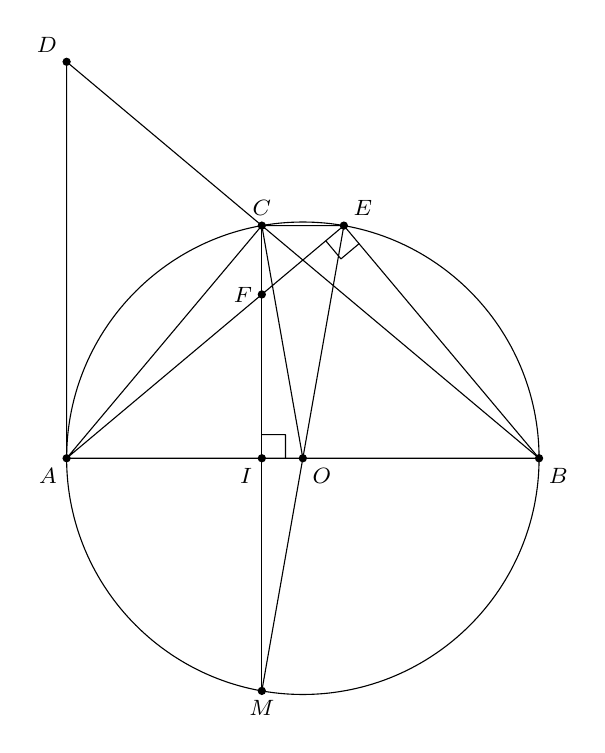
\begin{tikzpicture}[line join = round, line cap=round,>=stealth,font=\footnotesize,scale=1]
			\usetikzlibrary{calc,intersections,angles}
			
			% Khai báo hằng số
			\def\r{3} % r = 3cm
			\def\aConstant{4} % a = 4 (Lưu ý: hằng số a này không được sử dụng trong các định nghĩa điểm mới)
			\def\alphaAngle{100} % alpha = 100 độ
			
			% Định nghĩa tọa độ các điểm
			\coordinate (O) at (0,0);
			\coordinate (A) at (-\r,0);
			\coordinate (B) at (\r,0);
			% D(-r; 2r*tan(90-alpha/2))
			\pgfmathsetmacro{\yDVal}{2*\r*tan(90-\alphaAngle/2)}
			\coordinate (D) at (-\r,\yDVal);
			
			% Tọa độ cực C(alpha;r), E(80;r)
			\coordinate (C) at (\alphaAngle:\r);
			\coordinate (E) at (80:\r);
			
			% I là hình chiếu của C lên AB (trục Ox)
			% Cx = r*cos(alphaAngle), Cy = r*sin(alphaAngle)
			% Ix = Cx, Iy = 0
			\pgfmathsetmacro{\CxVal}{\r*cos(\alphaAngle)}
			\pgfmathsetmacro{\CyVal}{\r*sin(\alphaAngle)}
			\coordinate (I) at (\CxVal,0);
			
			% Lấy điểm M sao cho I là trung điểm của CM
			% Mx = 2*Ix - Cx = Ix
			% My = 2*Iy - Cy = -Cy
			\coordinate (M) at (\CxVal,-\CyVal);
			
			% AE cắt CM tại F
			\path[name path=lineAE_F] (A) -- (E);
			\path[name path=lineCM_F] (C) -- (M);
			\path[name intersections={of=lineAE_F and lineCM_F, by=F}];
			
			% Vẽ các đối tượng hình học
			\draw (O) circle (\r);          % Đường tròn (O;r)
			\draw (A) -- (D) -- (B) -- cycle; % Tam giác ADB (A-D-B-A)
			\draw (C) -- (M);               % Đoạn C-M
			\draw (O) -- (C);               % Đoạn O-C
			\draw (B)--(E)--(A) -- (C) -- (E) -- (M); % Đường A-C-E-M (Lưu ý: không đóng thành cycle)
			
			% Tô màu cho các điểm (theo cấu trúc đầu tiên)
			\fill (O) circle (1.5pt);
			\fill (A) circle (1.5pt);
			\fill (B) circle (1.5pt);
			\fill (D) circle (1.5pt);
			\fill (C) circle (1.5pt);
			\fill (E) circle (1.5pt);
			\fill (I) circle (1.5pt);
			\fill (M) circle (1.5pt);
			\fill (F) circle (1.5pt);
			
			% Đặt nhãn cho các điểm (theo cấu trúc đầu tiên)
			\node[below right] at (O) {$O$};
			\node[below left] at (A) {$A$};
			\node[below right] at (B) {$B$};
			\node[above left] at (D) {$D$};
			\node[above] at (C) {$C$}; % Vị trí tương đối
			\node[above right] at (E) {$E$}; % Vị trí tương đối
			\node[below left] at (I) {$I$};
			\node[below] at (M) {$M$}; % Vị trí tương đối
			\node[left] at (F) {$F$};   % Vị trí tương đối
			
			% Không có yêu cầu ký hiệu góc vuông trong lần này
			\pic[draw, angle radius=3mm]{right angle = F--I--B};
			\pic[draw, angle radius=3mm]{right angle = F--E--B};
		\end{tikzpicture}
		
		\end{center}
		}
\end{ex}

\begin{ex}
 Một người muốn làm một thùng tôn dạng khối hộp chữ nhật không nắp có thể tích bằng $288\text{dm}^3$. Đáy thùng là hình chữ nhật gấp đôi chiều rộng. Giá tôn làm thùng là 500000 đồng/m$^2$. Nếu người đó biết xác định các kích thước của thùng hợp lý thì chi phí cho việc mua tôn sẽ thấp nhất. Hỏi người đó trả chi phí thấp nhất để mua tôn làm thùng là bao nhiêu (giả sử các mép tôn hàn không đáng kể)?
	\loigiai{
	Gọi $x, y, h$ (m) lần lượt là chiều rộng, chiều dài đáy và chiều cao của hình hộp chữ nhật ($x, y, h > 0$).
	
	Theo bài ra ta có: $y = 2x$ và $xyh = 0,288$.
	
	Từ đó suy ra $h = \frac{0,144}{x^2}$.
	
	Diện tích tôn cần là: $S = xy + 2xh + 2yh = 2x^2 + \frac{0,864}{x} = 2(x^2 + \frac{0,432}{x}) = 2(x^2 + \frac{0,216}{x} + \frac{0,216}{x}) \ge 2 \cdot 3 \sqrt[3]{x^2 \cdot \frac{0,216}{x} \cdot \frac{0,216}{x}} = 2,16$ (Áp dụng BĐT Cô-si cho 3 số dương).
	
	$S \ge 2,16$ m$^2$.
	
	Vậy chi phí thấp nhất để mua tôn là: $2,16 \cdot 500000 = 1080000$ đồng.
	}
\end{ex}
\begin{ex}
	Cho ba số dương $a,b,c$ thỏa mãn $a+b+c=12$.
	Chứng minh rằng: $\frac{a}{b^2+16}+\frac{b}{c^2+16}+\frac{c}{a^2+16} \ge \frac{3}{8}$.
	\end{ex}
	
\setcounterref{ex}{0}
